\chapter{Self-Localization}\label{Chap:PF}
This chapter introduces the concrete method used in the current framework for NAO, the mobile roboter lacalization. RoboCup self-localization is a problem that NAO robot could determine its pose, which includes both position and angular, relative to the given map of the standard soccer field. Almost all the tasks for each robot player require knowledge of its pose on the field. We call this problem as rather a self-localization than a SLAM(Simultaneous localization and mapping) problem, one important reason is the map of the environment has been provided as prior knowledges. Self-localization could be treated as a problem of coordinate transformation. Map of the field or environment is described as the global coordinate system, which does not rely on robot's pose. The robot pose will be finally transformed into the global frame and represented as a global coordiante\cite{thrun2005probabilistic}. In our project the NAO pose is only changes in a plane, the $z$ element is always remains as zero since the robot always stands firmly on the ground. So the pose could be written as $(x,y,\theta)^T$.

However, the pose of robot could not be aquired directly, instead it could be inferred from the sensor data, which here come from camera. The sensor could not be hundred percentage accurate, it alway contains noise, especially image processing by using camera. So we have to find a proper method to calculate the pose from imperfect sensor data, which will be introduced in this chapter.

\section{General Framework: Particle Filter}
For self-localization, B-Human uses a particle filter based on the Monte Carlo method \cite{fox1999monte} as it is a proven approach to provide accurate results in such an environment \cite{rofer2005particle}. The reason for selecting particle filter in this self-localization problem is that in the RoboCup soccer match the robot will from time to time fall down, and then it will not get the correct knowledge of its position. The problem is that the robot might believe it knows where it is while it does not. This is called kidnapped robot problem \cite{thrun2005probabilistic}. So the particle filter will be adopted to solve this kidnapped robot problem and it does not demand initial position of robot.

The particle filter is a kind of bayes filter, based on Monte Carlo method. It uses several samples as particles to describe the posterior. In particle filter, the samples of a posterior distribution are called particles are represented as \cite{thrun2005probabilistic}: 
\[
\mathcal{X}_t:=x_t^{[1]},x_t^{[2]} \dots x_t^{[M]}
\]
The posterior of each particle $x_t^{m} (with 1 \leq m \leq M)$ is the probalbilty of the state at specigic time $t$. Usually, M, the number of the particles is very large to get a as perfect as possible approxiamtion, since particle filter is a non-parametrical method to estimate the state updating. However in the RoboCup situation, only 12 to 16 particles are adopted. Because the memory space and computaion speed are both limited on the robot NAO. During the match, it has a high demanding on instantaneity. Here I have not tested or verified the effectiveness of the so small number of samples. But in recent years B-Human team even drop the particles from 16 to 12 \cite{BHumanCodeRelease2010} and it is proven in practice which shows a great robustness and outstanding performance. Then how does robot NAO apply particle filter to localize itself is shown in the flowchart \fref{Ffc.sub.1}.
\begin{figure}[tbp]
\centering
\subfigure[Particle filter]{
\label{Ffc.sub.1}
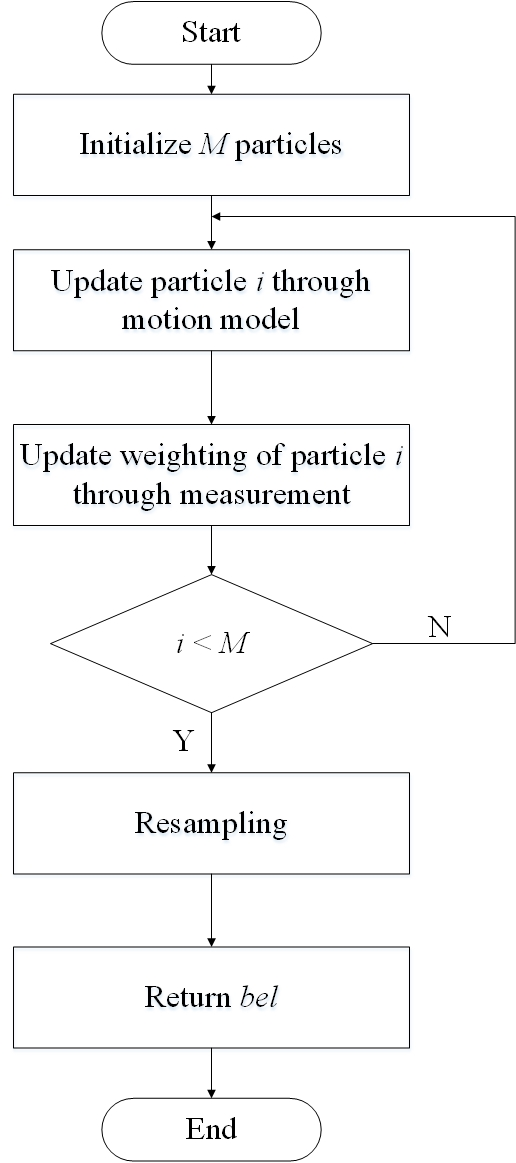
\includegraphics[width=0.3\textwidth]{pics/PF.jpg}}
\subfigure[combination of a PF and UKF]{
\label{Ffc.sub.2}
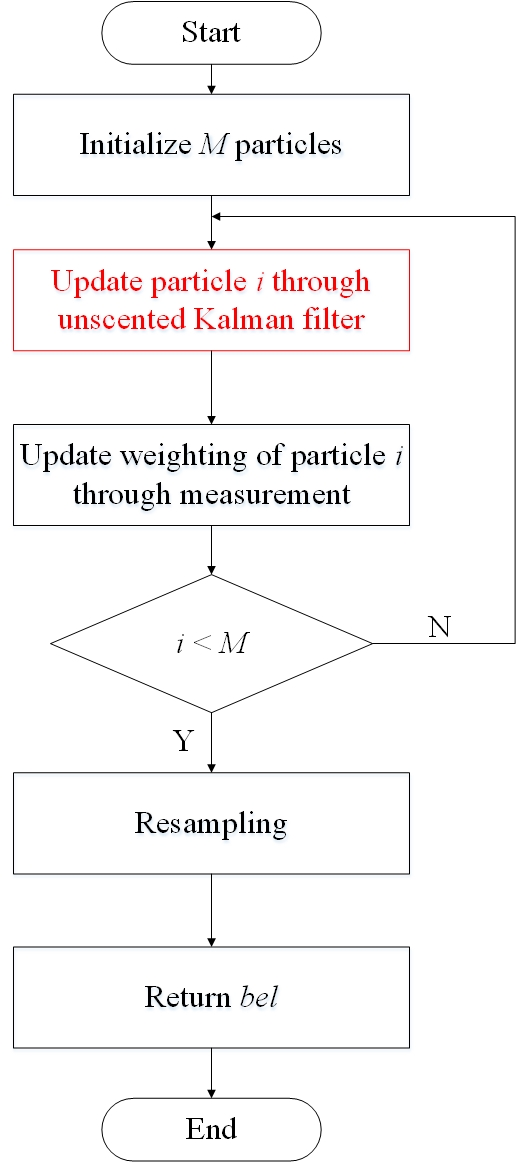
\includegraphics[width=0.3\textwidth]{pics/cpf.jpg}}
\caption{Self-localization based on particle filter flowchart}
\label{ffc}
\end{figure}

\section{Unscented Kalman Filter}
Since 2012, B-Human framewrok made a big change on self-localization: a combination of a particle filter and an Unscented Kalman filter is used.
The former computes a global position estimate; the latter performs local tracking for refining the global estimate \cite{BHumanCodeRelease2012}. 
This implementation will improve the local accuracy of particle filter and further results in improvement of localization precision. The change has shown in the \fref{Ffc.sub.1}. 

The idea behind the Unscented Kalman filter is similar to the original Kalman filter. However it is applied for the non-linear motion model and provides priciser result than Extented Kalman filter which uses first order approximation of Talor seires. It generates sigma points and uses the unscented transform to describe the non-linearity. The mean as well as covariance of states will also be modified with measurement and finally be returned.
